\documentclass[../template]{subfiles}

\begin{document}
\section{Shortest Path}
\subsection{Algoritmo di Dijkstra}
Applicabile soltanto nel caso in cui i pesi degli archi siano sempre non negativi.

\begin{center}
    \begin{tikzpicture}[rotate=90]
        \Vertices[unit=2.1]{circle}{0, 1, 2, 3}
        \tikzset{EdgeStyle/.style={->, bend right=18}}
        \Edge[label=$3$, color=red](0)(1)
        \Edge[label=$12$](0)(2)
        \Edge[label=$16$](0)(3)
        \Edge[label=$9$](1)(0)
        \Edge[label=$18$](1)(2)
        \Edge[label=$7$, color=red](1)(3)
        \Edge[label=$5$](2)(0)
        \Edge[label=$3$, color=red](2)(3)
        \Edge[label=$8$](3)(0)
        \Edge[label=$1$](3)(2)
        ;
    \end{tikzpicture}
\end{center}
\lstinputlisting{algorithms/dijkstra.py}
\subsubsection{Dimostrazione Correttezza}
%48m lezione 5
\end{document}
